\subsection{Research Objective and Translational Framework}

The objective of this study was to determine whether the available evidence
supports a scientifically defensible first-generation pathway for real-time
closed-loop Targeted Memory Reactivation (TMR). Its principal methodological
contribution is a traceable process for translating findings from neuroscience,
sleep research, wearable sensing, and closed-loop intervention into
system-level requirements and a justified implementation direction.

The analysis distinguished four translational levels that are related but not
interchangeable:

\begin{enumerate}
    \item \textbf{Biological plausibility}: whether the proposed intervention is
    consistent with established mechanisms of memory formation, sleep-dependent
    consolidation, sensory processing, and neural reactivation;

    \item \textbf{Experimental efficacy}: whether the intervention produces
    measurable effects under controlled conditions;

    \item \textbf{Technical feasibility}: whether available sensing,
    computation, and intervention technologies can reproduce the functions
    required by the experimental paradigm; and

    \item \textbf{Product readiness}: whether an integrated system demonstrates
    sufficient reliability, safety, usability, and generalizability for
    deployment.
\end{enumerate}

These levels define the translational boundary of the study. Biological
plausibility does not establish experimental efficacy; experimental efficacy
does not guarantee technical feasibility; and technical feasibility does not
demonstrate product readiness. Conclusions were therefore restricted to the
level directly supported by the reviewed evidence.

The investigation integrated six evidence domains:

\begin{enumerate}
    \item mechanisms of learning, memory formation, and consolidation;
    \item sleep-dependent memory processing and neural reactivation;
    \item experimental evidence for TMR;
    \item wearable and portable sleep-monitoring technologies;
    \item real-time sleep-state estimation; and
    \item closed-loop physiological intervention.
\end{enumerate}

These domains form a constraint chain rather than an independent checklist.
Memory and sleep neuroscience define the physiological conditions relevant to
TMR. Measurement research determines whether those conditions are observable
through a candidate sensing modality. Real-time analysis determines whether the
required information can be obtained during ongoing sleep, while closed-loop
research determines whether that information can govern cue delivery without
unacceptable disturbance. The evidence supporting each stage consequently
limits the claims that can be made about the stages that follow it.

Each domain was examined only to the depth required by this translation problem.
Foundational neuroscience was limited to memory encoding, hippocampal--
neocortical consolidation, sleep-dependent reactivation, sensory cue processing,
and electrophysiological activity relevant to sleep monitoring. The technology
analysis emphasized electroencephalography (EEG) and
photoplethysmography (PPG), representing the principal electrophysiological and
peripheral sensing pathways evaluated in this study. Actigraphy, cardiac
measures, respiration, temperature, and other modalities were considered where
they informed the interpretation of EEG-, PPG-, or multimodal systems.

A governing principle of the analysis was that measurement performance must be
interpreted relative to its intended closed-loop function. Agreement with
retrospective sleep staging does not by itself demonstrate that a sensing system
can support causal state estimation, bounded decision latency, uncertainty
handling, intervention control, or post-cue monitoring. General-purpose
performance was therefore not treated as equivalent to intervention readiness.

The endpoint of the present study was an evidence-derived set of translational
requirements and a justified first-generation implementation pathway. Detailed
signal-processing development, machine-learning model training, software
architecture, hardware integration, numerical latency thresholds, usability
testing, longitudinal or clinical validation, regulatory analysis, and
commercial evaluation were reserved for subsequent engineering and experimental
work.


\subsection{Evidence Identification and Source Selection}

The study employed a structured, question-driven translational evidence
synthesis. This design was selected because the research problem required the
integration of heterogeneous forms of evidence serving different functions:
mechanistic findings, experimental effects, measurement-validation results,
real-time feasibility studies, and implementation constraints. The purpose was
not to calculate a new pooled effect or exhaustively map a single literature,
but to determine how evidence from several domains constrains a specific
technology-development pathway.

The study should therefore not be interpreted as a formal systematic review,
scoping review, or meta-analysis. Such review designs differ in purpose,
retrieval requirements, appraisal procedures, and permissible conclusions
\citep{grant2009typology,snyder2019literature}. The present synthesis was
organized around bounded research questions and prioritized evidential relevance
and claim-to-decision traceability rather than exhaustive publication retrieval.

For each research question, sources were retained when they served at least one
of the following functions:

\begin{itemize}
    \item establishing a biological or physiological mechanism relevant to TMR;
    \item quantifying the efficacy, variability, or boundary conditions of TMR;
    \item validating a measurement method or wearable sensing modality;
    \item evaluating real-time or closed-loop operation;
    \item identifying a limitation affecting translation beyond the laboratory;
    or
    \item constraining or distinguishing a system-level implementation decision.
\end{itemize}

The evidence base included foundational neuroscience and sleep-medicine texts,
peer-reviewed reviews and meta-analyses, primary experimental studies,
independent wearable-validation studies, and technical literature related to
real-time physiological monitoring. Primary studies were preferred for specific
experimental findings and device-performance claims. Reviews and
meta-analyses were used to evaluate effect magnitude, consistency,
heterogeneity, and broader evidentiary boundaries. Recent empirical studies were
prioritized in rapidly developing fields such as wearable sensing, automated
sleep analysis, and home-based intervention, while authoritative texts and
widely cited reviews were retained for comparatively stable foundational
concepts.

Manufacturer documentation was consulted only when needed to establish publicly
reported sensor configurations, device functions, data-access capabilities, or
integration provisions. Manufacturer-reported performance was not treated as
independent evidence of measurement accuracy, TMR efficacy, or closed-loop
readiness. Wherever possible, device-performance claims were based on
peer-reviewed comparisons with polysomnography or another appropriate
physiological reference.

Sources were excluded from the central synthesis when they lacked direct
relevance to a research question, duplicated conclusions already supported by
stronger evidence, relied primarily on promotional claims, or could not inform a
scientific or translational decision. Wearable-validation findings were treated
cautiously when their populations, recording conditions, output definitions, or
temporal assumptions differed substantially from the intended closed-loop
function.

Source identification, appraisal, and synthesis were conducted by a single
reviewer. Procedural safeguards included the use of predefined research
questions, explicit source-function criteria, preference for primary and
independently validated evidence, conservative treatment of conflicting
findings, and traceability between each retained source and the research
question it informed. Each source was mapped within the supporting Neuro-TMR
research repository to preserve the connection between literature,
interpretation, translational requirement, and implementation decision.

These procedures reduced unrestricted source selection but did not eliminate
reviewer-dependent judgment. Duplicate screening, formal risk-of-bias scoring,
standardized certainty grading, and a new quantitative synthesis were not
performed. Quantitative effect estimates were therefore taken from published
meta-analyses or individual studies rather than recalculated across the assembled
literature.


\subsection{Evidence Appraisal and Maturity Classification}

The selected evidence was evaluated according to its strength, relevance, and
translational value rather than publication count alone. Appraisal considered
six dimensions:

\begin{itemize}
    \item \textbf{Methodological validity}: study design, participant
    characteristics, control conditions, measurement methods, statistical
    reporting, and outcome definitions;

    \item \textbf{Consistency and replication}: convergence across independent
    studies, laboratories, populations, and experimental paradigms;

    \item \textbf{Effect magnitude and uncertainty}: reported effect sizes,
    confidence intervals, interindividual variability, and the distinction
    between statistical and practical significance;

    \item \textbf{Physiological specificity}: how directly a measurement or
    intervention represented the biological process required by the proposed
    closed-loop function;

    \item \textbf{Ecological validity}: the extent to which findings obtained
    under controlled conditions remained applicable to wearable, home-based, or
    unsupervised operation; and

    \item \textbf{Translational relevance}: whether a finding could constrain a
    system requirement, distinguish candidate pathways, or define a future
    validation question.
\end{itemize}

These dimensions informed qualitative critical appraisal; they were not
converted into a numerical quality score. A methodologically strong study could
still have limited translational relevance if its measurement, timing, or
operational conditions differed substantially from those required for
closed-loop TMR. Conversely, a study with narrow scope could remain
translationally important if it directly tested a critical system assumption.

Conflicting findings were examined in relation to differences in participant
characteristics, memory task, cue modality, cue intensity, sleep stage, sensing
technology, study duration, and outcome definition. Disagreement was not
resolved through simple frequency counting. When evidence remained
heterogeneous or insufficiently replicated, the conclusion was restricted to
the conditions directly supported by the literature.

Evidence maturity was classified separately from the four translational levels
defined in Section~2.1. The translational levels specify the type of claim being
made, whereas the maturity categories indicate how strongly that claim is
supported.

\begin{itemize}
    \item \textbf{Established evidence}: findings supported by convergent
    experimental results, independent replication, authoritative reviews or
    meta-analyses, or validated measurement methods;

    \item \textbf{Preliminary evidence}: findings supported by a limited number
    of studies, early home-based demonstrations, narrow populations, short
    study durations, or incomplete independent replication; and

    \item \textbf{Unresolved evidence}: claims for which mechanism,
    measurement validity, implementation performance, or intervention efficacy
    remained insufficient to support a first-generation system assumption.
\end{itemize}

These categories were interpretive rather than formal statistical grades. Their
purpose was to prevent preliminary feasibility from being represented with the
same confidence as convergent experimental evidence.

The appraisal also maintained a distinction between measurement accuracy and
functional suitability. A sleep-staging system may achieve acceptable
retrospective classification performance while remaining unsuitable for
real-time intervention because of delayed output, inadequate signal-quality
assessment, uncertain confidence calibration, restricted access to raw data, or
inability to detect post-cue physiological changes. Performance claims were
therefore interpreted in relation to the decision the sensing system was
expected to support.

The output of this stage was an evidence-bounded conclusion for each research
question. Each conclusion documented the strongest supported interpretation,
the conditions under which it remained valid, the principal sources of
uncertainty, and any assumption requiring subsequent experimental validation.


\subsection{Evidence-to-Engineering Translation}

The central methodological unit linked each scientific conclusion to a
prospective engineering decision through four operations:

\begin{enumerate}
    \item \textbf{Evidence-bounded conclusion}: the strongest interpretation
    supported by the literature, together with its conditions and limitations;

    \item \textbf{Functional implication}: the capability a practical system
    would require for that conclusion to remain operationally relevant;

    \item \textbf{System-level requirement}: a testable requirement describing
    what the system must measure, detect, control, or prevent; and

    \item \textbf{Validation question}: an unresolved assumption that must be
    examined during engineering or experimental development.
\end{enumerate}

For example, the evidence indicates that TMR cueing should occur during
physiologically appropriate sleep conditions while avoiding arousal and sleep
disruption. The functional implication is that a practical system must
distinguish eligible intervals from unstable or unsuitable periods. The
corresponding system-level requirement is that the controller must use ongoing
physiological information to authorize, withhold, or suspend cue delivery. The
remaining validation question is whether a selected sensing and control pathway
can support these decisions reliably during overnight operation.

This intermediate translation prevents biological findings from being converted
directly into a specific device, algorithm, or numerical threshold. A
physiological function may potentially be implemented through more than one
sensing modality. Candidate technologies were therefore compared only after the
required function had been defined.

Figure~\ref{fig:research_workflow} summarizes the complete six-stage workflow.

\begin{figure*}[t]
    \centering
    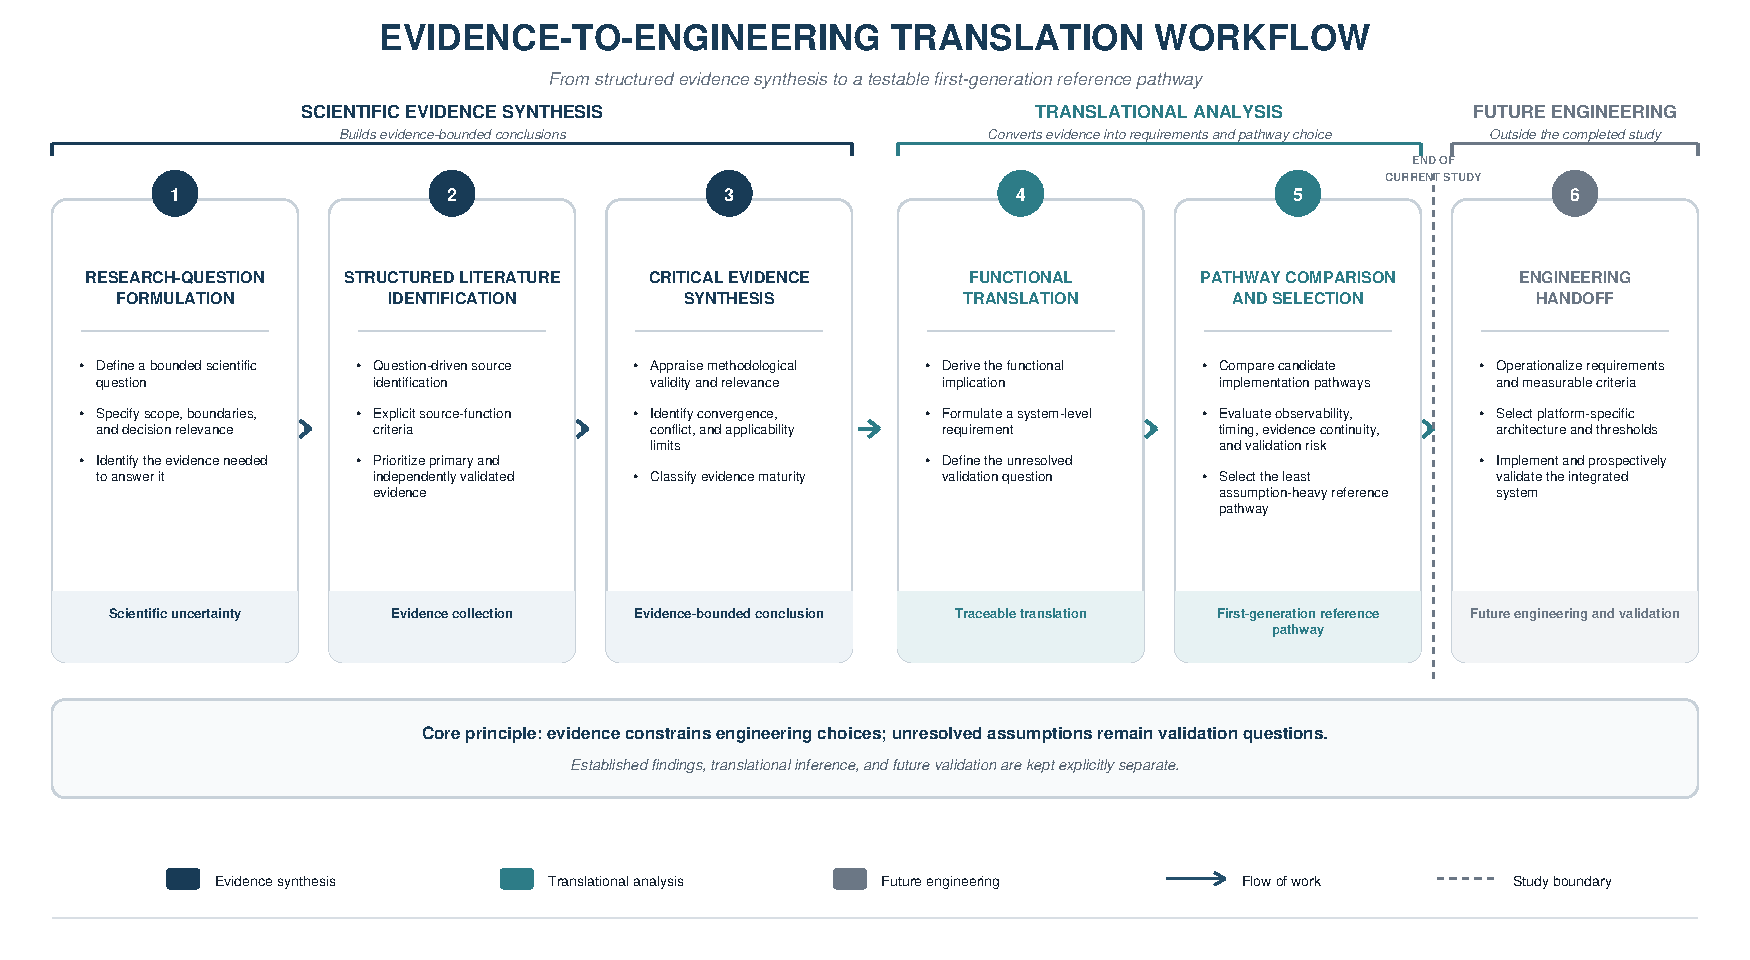
\includegraphics[width=\textwidth]
    {figures/fig1_research_workflow.pdf}
    \caption{
Evidence-to-engineering translation workflow used in this study.
Steps 1--3 formulate bounded research questions, identify relevant
literature through a structured question-driven process, and produce
evidence-bounded conclusions. Step~4 translates those conclusions into
functional implications, system-level requirements, and unresolved
validation questions. Step~5 compares candidate implementation pathways
and selects the first-generation reference pathway according to
physiological observability, evidentiary continuity, temporal suitability,
and validation risk. Step~6 represents the subsequent engineering and
prospective validation program and lies outside the completed scope of
the present study. Unresolved assumptions are retained as validation
questions rather than converted into predetermined engineering
specifications. The figure is an original methodological synthesis by
the author.
}
    \label{fig:research_workflow}
\end{figure*}

The six stages were:

\begin{enumerate}
    \item \textbf{Research-question formulation.}
    Each investigation began with a bounded question specifying the phenomenon,
    the evidence needed to evaluate it, and its relevance to the overall
    translation problem.

    \item \textbf{Structured literature identification.}
    Sources were selected according to their ability to establish a mechanism,
    quantify an effect, validate a measurement method, identify a limitation,
    or constrain a translational decision.

    \item \textbf{Critical evidence synthesis.}
    Findings were evaluated across studies to identify convergence,
    disagreement, applicability boundaries, methodological limitations, and
    unresolved uncertainty.

    \item \textbf{Functional translation.}
    Each evidence-bounded conclusion was reformulated as a statement of what a
    practical closed-loop system would need to accomplish.

    \item \textbf{Pathway comparison and selection.}
    Candidate implementation pathways were evaluated against the derived
    requirements according to physiological relevance, temporal suitability,
    evidence maturity, operational burden, and validation risk.

    \item \textbf{Engineering handoff.}
    The selected pathway and unresolved assumptions were transferred into a
    future program of component development, integration, prospective testing,
    and iterative refinement.
\end{enumerate}

The resulting requirement set covered seven areas:

\begin{itemize}
    \item \textbf{Physiological eligibility}: the states and conditions under
    which cueing may be appropriate;

    \item \textbf{Measurement quality}: the signal observability, reliability,
    physiological specificity, and uncertainty information required to support
    a decision;

    \item \textbf{Temporal validity}: the need for causal estimates, measurable
    processing delay, synchronized cue execution, and appropriately bounded
    intervention timing;

    \item \textbf{Intervention control}: the conditions under which cues must be
    delivered, withheld, modified, or terminated;

    \item \textbf{Disturbance prevention}: the detection and reduction of
    arousal, sleep disruption, inappropriate stimulation, or other unintended
    effects;

    \item \textbf{Operational reliability}: signal-quality monitoring,
    repeatability, fail-safe behavior, and robustness outside controlled
    laboratory conditions; and

    \item \textbf{Empirical validation}: the prospective tests required before
    an implementation assumption can be treated as a demonstrated capability.
\end{itemize}

Candidate pathways were evaluated according to how directly and reliably they
could satisfy these functions. Commercial availability, comfort, or
general-purpose sleep-staging performance were not sufficient grounds for
selection when the corresponding closed-loop function remained unsupported.
Where the evidence did not permit a definitive translation, uncertainty was
retained as a validation requirement rather than resolved through technological
preference.


\subsection{Study Outputs and Methodological Boundary}

The methodology produced four outputs:

\begin{enumerate}
    \item evidence-bounded conclusions concerning memory consolidation, TMR,
    wearable sensing, and closed-loop intervention;

    \item an evidence-derived set of system-level translational requirements;

    \item a structured comparison of candidate first-generation implementation
    pathways; and

    \item selection of the pathway with the strongest continuity with the
    established evidence and the fewest unsupported assumptions.
\end{enumerate}

These outputs define a scientifically justified starting point for subsequent
development. They do not constitute evidence that an integrated system has been
implemented, that its operating parameters have been determined, or that it
produces reliable memory benefits outside the conditions represented in the
reviewed literature.

The methodological conclusions are also bounded by the question-driven,
single-reviewer design. The synthesis did not provide exhaustive literature
retrieval, duplicate screening, formal risk-of-bias grading, or a new
meta-analysis. These limitations reduce the certainty with which the resulting
pathway can be generalized and are examined further in Section~7.

The present study therefore ends at pathway selection and qualitative
requirement definition. Subsequent work must operationalize the requirements,
select platform-specific architectures and thresholds, implement the
closed-loop system, and evaluate its physiological reliability, behavioral
efficacy, safety, and generalizability. The selected first-generation pathway
should be interpreted as a testable development hypothesis rather than as a
completed architecture or validated memory-enhancement product.